\documentclass[letterpaper,11pt]{article}
\oddsidemargin -1.0cm \textwidth 17.5cm

\usepackage[utf8]{inputenc}
\usepackage[activeacute,spanish]{babel}
\usepackage{amsfonts,setspace}
\usepackage{amsmath}
\usepackage{amssymb, amsmath, amsthm}
\usepackage{comment}
\usepackage{float}
\usepackage{amssymb}
\usepackage{dsfont}
\usepackage{anysize}
\usepackage{multicol}
\usepackage{enumerate}
\usepackage{graphicx}
\usepackage[left=1.5cm,top=1.5cm,right=1.5cm, bottom=1.7cm]{geometry}
\setlength\headheight{1.5em} 
\usepackage{fancyhdr}
\usepackage{multicol}
\usepackage{hyperref}
\usepackage{wrapfig}
\usepackage{subcaption}
\pagestyle{fancy}
\fancyhf{}
\renewcommand{\labelenumi}{\normalsize\bfseries P\arabic{enumi}.}
\renewcommand{\labelenumii}{\normalsize\bfseries (\alph{enumii})}
\renewcommand{\labelenumiii}{\normalsize\bfseries \roman{enumiii})}

\begin{document}

\fancyhead[L]{\itshape{Facultad de Ciencias F\'isicas y Matem\'aticas}}
\fancyhead[R]{\itshape{Universidad de Chile}}

\begin{minipage}{11.5cm}
    \begin{flushleft}
        \hspace*{-0.6cm}\textbf{FI1100-6 Introducción a la Física Moderna}\\
        \hspace*{-0.6cm}\textbf{Profesor:} Diego Mardones\\
        \hspace*{-0.6cm}\textbf{Auxiliares:} Gabriel O\textsc{\char13}Ryan, Camila Sepúlveda, Alejandro Silva\\
        \hspace*{-0.6cm}\textbf{Ayudante:} Sebastián Vargas
    \end{flushleft}
\end{minipage}

\begin{picture}(2,3)
    \put(366, 10){
\includegraphics[scale=0.9]{Imágenes/logo/dfi-fcfm.pdf}}
\end{picture}

\begin{center}
	\LARGE\textbf{Auxiliar \#6:}\\
	\Large{Óptica Geométrica}
\end{center}

\vspace{-1cm}
\begin{enumerate}\setlength{\itemsep}{0.4cm}

\rfoot[]{pág. \thepage}

\item[]

\item Imagina que eres un pez en el fondo de un lago con un líquido desconocido. Al alzar la vista en un ángulo $\alpha = 32^{\circ}$ con respecto a la vertical observas una gaviota. Por interno te avisan que la luz proveniente de la gaviota tiene un ángulo de incidencia $\beta = 49^{\circ}$.

\begin{enumerate}
    \item ¿Cuál es el índice de refracción de este líquido en el cual estás nadando?
    
    \item Nuevamente, por interno, te avisan que hay otra gaviota cerca y que para verla tienes que mirar en un ángulo $\gamma = 47^{\circ}$ con respecto a la vertical. ¿Realmente se podrá ver? ¿Por qué?
\end{enumerate}

\begin{figure}[H]
    \centering
    \begin{subfigure}[t]{0.5\textwidth}
        \centering
        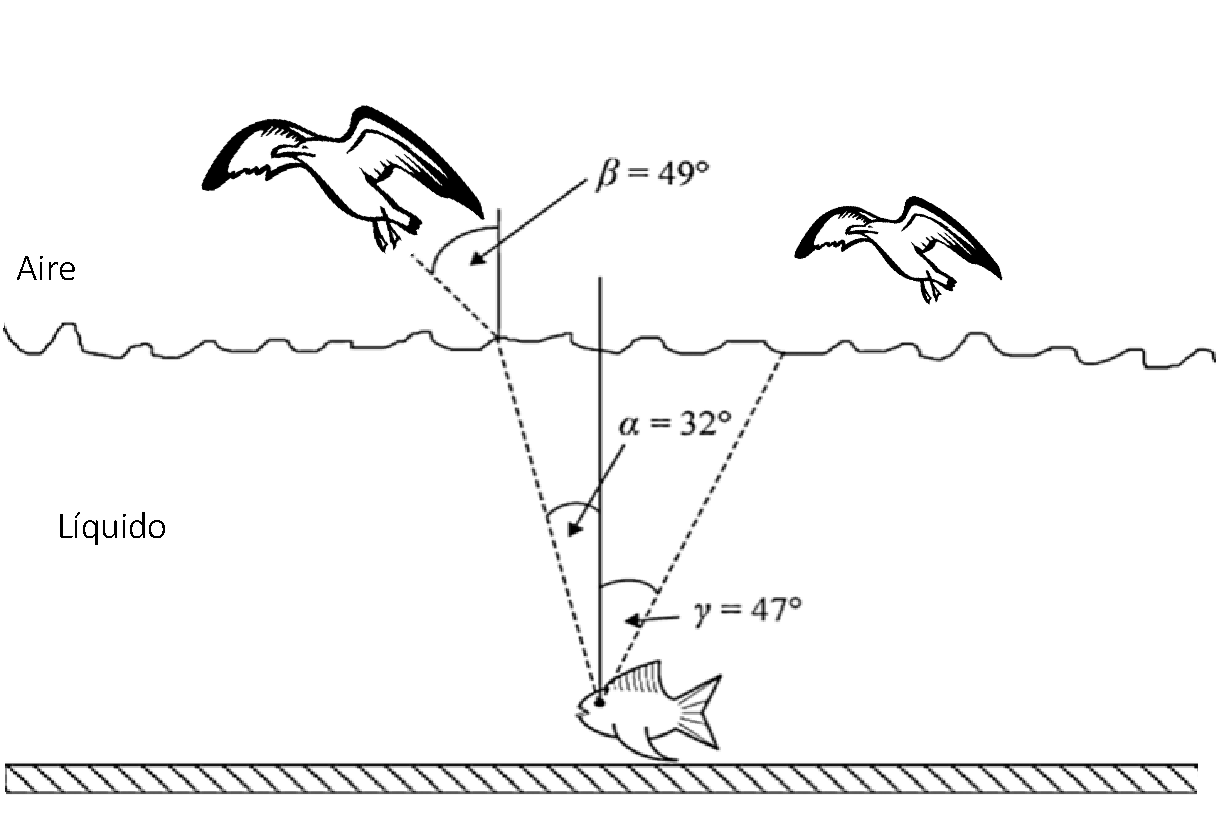
\includegraphics[width = 0.7\linewidth]{Imágenes/aux6/pajaros.pdf}
        \caption*{Figura P1}
    \end{subfigure}
    \hspace{0.5cm}
    \begin{subfigure}[t]{0.4\textwidth}
        \centering
        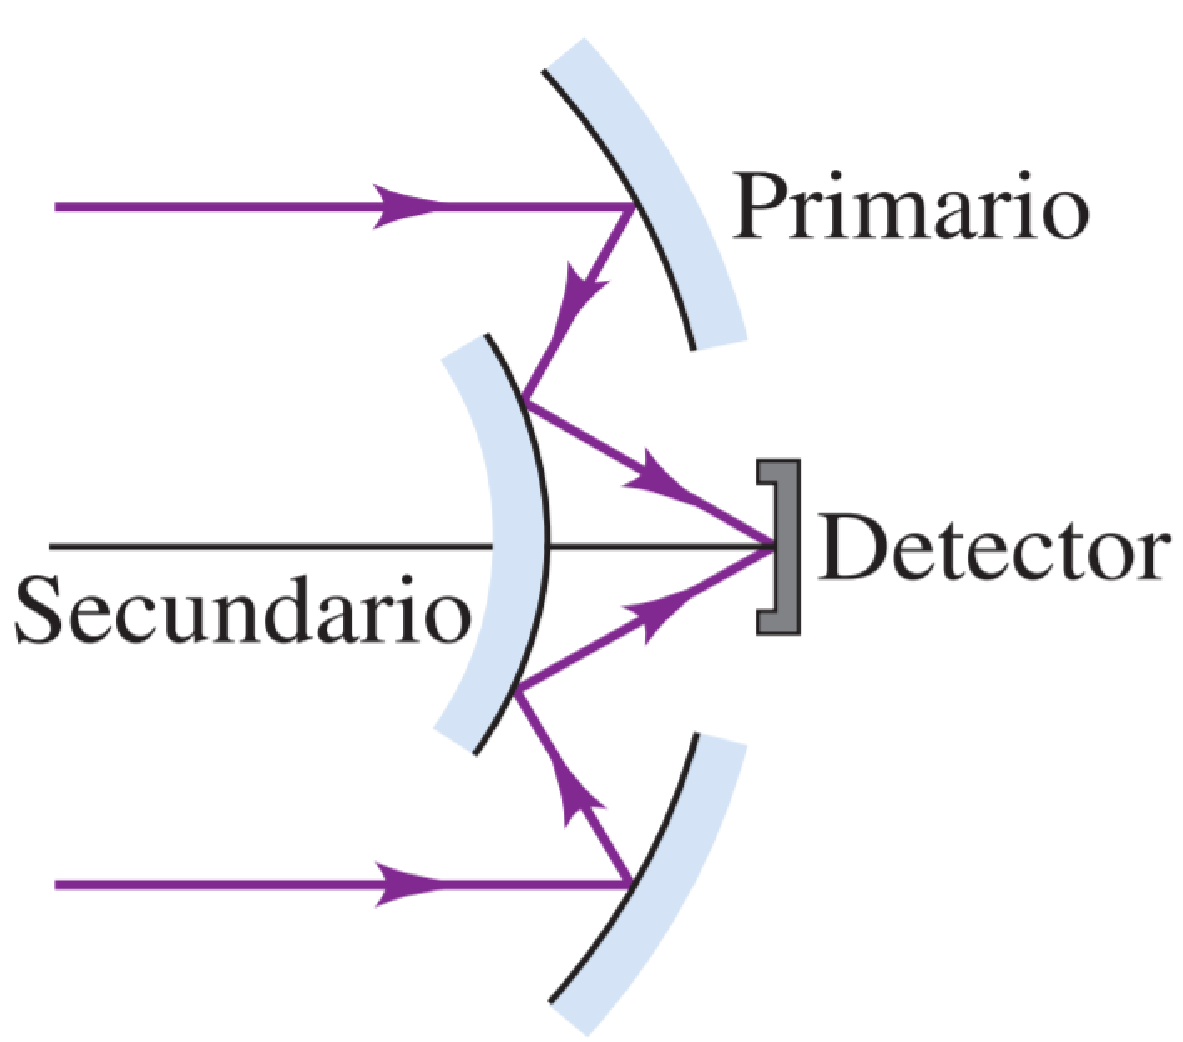
\includegraphics[width = 0.6\linewidth]{Imágenes/aux6/cas.pdf}
        \caption*{Figura P5}
    \end{subfigure}
\end{figure}

\item La imagen de un árbol cubre exactamente la longitud de un espejo plano de $4$ cm de alto, cuando el espejo se sostiene a $35$ cm del ojo. El árbol está a $28$ m del espejo. ¿Cuál es su altura?

\item Usted sostiene un tazón de ensalada esférico a $90$ cm frente a su cara, con el fondo del tazón hacia usted. El tazón es de metal pulido con un radio de curvatura de $35$ cm.

\begin{enumerate}
    \item ¿Dónde se localiza la imagen de su nariz de $2$ cm de largo?
    
    \item ¿Cuáles son el tamaño, la orientación y la naturaleza de la imagen?
\end{enumerate}

\item Se coloca un objeto de 0.6 cm de altura a 16.5 cm a la izquierda del vértice de un espejo esférico convexo, cuyo radio de curvatura es de 22 cm.

\begin{enumerate}
    \item Dibuje un diagrama de rayos principales para mostrar la formación de la imagen
    
    \item Determine la posición, el tamaño, la orientación y la naturaleza (real o virtual) de la imagen.
\end{enumerate}

\item Un telescopio reflectante del sistema Cassegrain utiliza dos espejos, el espejo secundario enfoca la imagen a través de un orificio en el espejo primario (ver Figura P5). Se desea enfocar la imagen de una galaxia distante en el detector de la figura. Si el espejo primario tiene una distancia focal de 2.5 m, el espejo secundario tiene una distancia focal de -1.5 m y la distancia entre el vértice del espejo primario y el detector es de 15 cm. ¿Cuál debería ser la distancia entre los vértices de los dos espejos?
\end{enumerate}
\end{document}